\textbf{Benötigte Komponenten für \hyperlink{lf-nn-01}{/LF03/}} \\

\paragraph{STM32 Nucleo-F722ZE}\mbox{}\\

\begin{wrapfigure}{r}{0.4\textwidth} % Increase the width of the figure environment
	\vspace{-10pt}
	\hspace{20pt}
	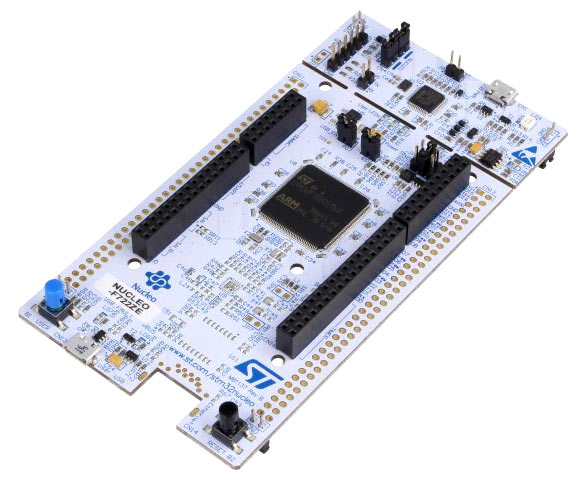
\includegraphics[width=0.25\textwidth]{images/05_technische_spezifikation/nn/nucleo_f722ze.jpg}
	\caption{STM32 Nucleo-F722ZE Board}
	\label{fig:nucleo-f722ze}
\end{wrapfigure}


Das in \textbf{Abbildung \ref{fig:nucleo-f722ze}} gezeigte STM32 Nucleo-F722ZE Board beinhaltet einen Microcontroller und wird in erster Linie für den Betrieb des neuronalen Netzes benötigt, auf ihm sollen allerdings das gesamte Projekt laufen. Nachdem noch keine Erfahrungen mit neuronalen Netzen auf Microcontrollern gesammelt wurden, wurde dieses Board ausgewählt, da es über mehr Ressourcen verfügt als die verfügbaren Nucleo-F7401RE Boards. Dadurch soll sicher gestellt werden, dass es im Projektverlauf nicht zu Ressourcenknappheiten, insbesondere beim RAM,  kommt.

Es verfügt im Vergleich zum STM32 Nucleo-F401RE Board über mehr SRAM (256 Kbytes vs. 96 Kbytes) und über eine leistungsstärkere CPU (Cortex M7 CPU mit 462 DMIPS/2.14 DMIPS vs. Cortex M4 CPU mit 105 DMIPS/1.25 DMIPS).
Das Board wird mit einer Versorgungsspannung von 5V betrieben. \cite{stm32F7-board}